%Notes by Harsh Mistry 
%Econ 301
%Based on Template From  https://www.cs.cmu.edu/~ggordon/10725-F12/template.tex

\documentclass[twoside]{article}
\setlength{\oddsidemargin}{0.25 in}
\setlength{\evensidemargin}{-0.25 in}
\setlength{\topmargin}{-0.6 in}
\setlength{\textwidth}{6.5 in}
\setlength{\textheight}{8.5 in}
\setlength{\headsep}{0.75 in}
\setlength{\parindent}{0 in}
\setlength{\parskip}{0.1 in}
\usepackage{amsmath,amsfonts,graphicx, color}
\usepackage{tikzsymbols}
\newcounter{lecnum}
\renewcommand{\thepage}{\thelecnum-\arabic{page}}
\renewcommand{\thesection}{\thelecnum.\arabic{section}}
\renewcommand{\theequation}{\thelecnum.\arabic{equation}}
\renewcommand{\thefigure}{\thelecnum.\arabic{figure}}
\renewcommand{\thetable}{\thelecnum.\arabic{table}}
\newcommand{\lecture}[4]{
   \pagestyle{myheadings}
   \thispagestyle{plain}
   \newpage
   \setcounter{lecnum}{#1}
   \setcounter{page}{1}
   
   
%Info Box 
   \begin{center}
   \framebox{
      \vbox{\vspace{2mm}
    \hbox to 6.28in { {\bf Econ 301 - Microeconomic Theory 2
	\hfill Winter 2018} }
       \vspace{4mm}
       \hbox to 6.28in { {\Large \hfill Lecture #1: #2  \hfill} }
       \vspace{2mm}
       \hbox to 6.28in { {\it Lecturer: #3 \hfill Notes By: #4} }
      \vspace{2mm}}
   }
   \end{center}
   
   \markboth{Lecture #1: #2}{Lecture #1: #2}



 
}

\renewcommand{\cite}[1]{[#1]}
\def\beginrefs{\begin{list}%
        {[\arabic{equation}]}{\usecounter{equation}
         \setlength{\leftmargin}{2.0truecm}\setlength{\labelsep}{0.4truecm}%
         \setlength{\labelwidth}{1.6truecm}}}
\def\endrefs{\end{list}}
\def\bibentry#1{\item[\hbox{[#1]}]}

\newcommand{\fig}[3]{
			\vspace{#2}
			\begin{center}
			Figure \thelecnum.#1:~#3
			\end{center}
	}
	
	\graphicspath{ {images/} }

\newtheorem{theorem}{Theorem}[lecnum]
\newtheorem{lemma}[theorem]{Lemma}
\newtheorem{ex}[theorem]{Example}
\newtheorem{proposition}[theorem]{Proposition}
\newtheorem{claim}[theorem]{Claim}
\newtheorem{corollary}[theorem]{Corollary}
\newtheorem{definition}[theorem]{Definition}
\newenvironment{proof}{{\bf Proof:}}{\hfill\rule{2mm}{2mm}}
\newcommand\E{\mathbb{E}}


%Start of Document 
\begin{document}

\lecture{17}{March 14, 2018}{Jean Guillaume Forand}{Harsh Mistry}


\section{Externalities Continued} 
\begin{ex} An example of a two-consumer economy with externalities
\begin{itemize}
\item Consumers have endowments \(\omega^A = (2,1)\) and \(\omega^B = (1, 1) \)
\item Consumer A has utility \(u^A(x_1^A, x_2^B) = x_1^{A \frac{1}{2}}x_2^{A\frac{1}{2}}\)
\item Consumer B has utility \(u^B(x_1^B, x_2^B) = x_1^{B\frac{1}{2}} [2-x_2^A]^{\frac{1}{2}}\)
\begin{itemize}
\item Consumption of good 2 imposes a negative externality on consumer B
\item Interpret \(x_2^A\) in utility function for B as aggregate amount of consumption of good 2 in the economy
\end{itemize}
\begin{center}
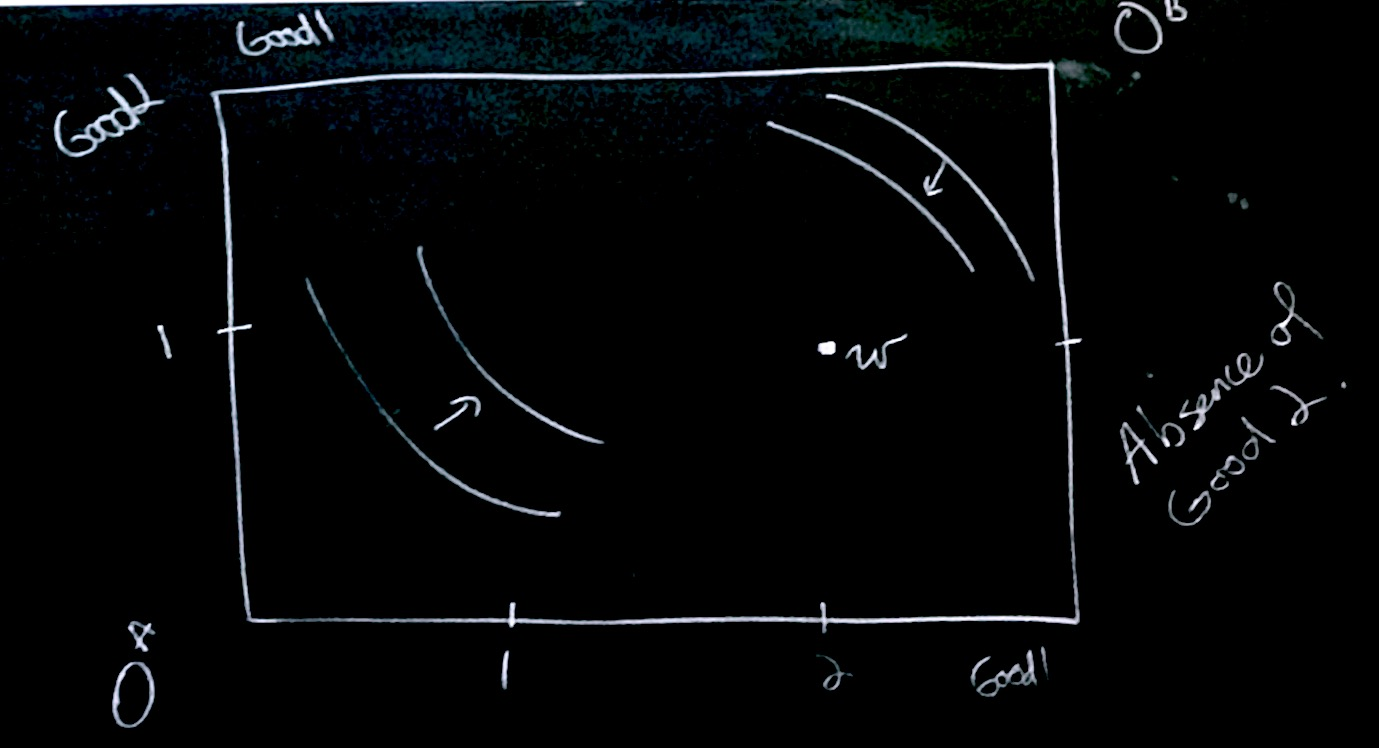
\includegraphics[scale=0.15]{30}
\end{center}
\item Find a competitive equilibrium of this economy
\item Demand functions:
\[(x_1^A (p), x_2^A(p)) = \left(\frac{2p_1+p_2}{2p_1}, \frac{2p_1+p_2}{2p_2}\right)\]
\[(x_1^B (p), x_2^B(p)) = \left(\frac{m}{p_1}, 0\right)\rightarrow  \text{ Consumer B only values good 1}\]
\item Normalize \(p_1^* = 1\), (MC2)
\[\frac{2+p_2^*}{2p_2^*} = 2 \implies p_2^* = \frac{2}{3}\]
\begin{itemize}
\item Prices \(p^* = (1 , \frac{2}{3})\) and allocations 
\(x^{A*} = \left(\frac{4}{3}, 2\right)\), \(x^{B*} = \left(\frac{5}{3}, 0\right)\) form a competitive equilibrium 
\end{itemize}
\item \(x^{A*}\) and \(x^{B*}\) are not pareto-efficient
\[\begin{aligned} 
\frac{\frac{d}{dx_1^{A*}} u^A(x_1^{A*}, x_2^{A*})}{\frac{d}{dx_2^{A*}} u^A(x_1^{A*}, x_2^{A*})} = \frac{x_2^{A*}}{x_1^{A*}} = \frac{3}{2}
\end{aligned}\]
\[\begin{aligned} 
\frac{\frac{d}{dx_1^{B*}} u^B(x_1^{A*}, x_2^{B*})}{\frac{d}{dx_2^{B*}} u^B(x_1^{A*}, x_2^{B*})} = \frac{2-x_2^{A*}}{x_1^{B*}} = 0
\end{aligned}\]
\item In equilibrium, consumer A consumes "too much" of good 2 relative to its impact on consumer B.
\item Consumer B is willing to exchange good 1 against reduction in consumption of good 2, but no market for this trade exists.  
\item FWT fails which is an example of a \underline{market failure}
\item Problem is that there is a missing market, as there is no market for the third good ("absence of good 2"), which is a good that consumer B values.
\item Can we restore efficiency in this market?
\item Solution 1 : compete the set of markets
\item Establish a market in which : 
\begin{itemize}
\item Consumer B can purchase right to be free of external effects of consumption of good 2.
\item Consumer A can purchase rights to produce externality
\item 3 markets: good 1, good 2, and rights to externalities generated by good 2 
\end{itemize}
\item Must specify what allocations of rights over externality 
\begin{itemize}
\item Fix endowments \(0 \leq \omega_R^A \leq 2 \) and \(\omega_R^B 2 - \omega^A_R\)
\end{itemize} 
\end{itemize}
\end{ex}
\begin{center}
\textcolor{blue}{Yes, we did spend the entire class on just one example. That's how long these problems take.}  \Sadey[1.3][red]
\end{center}


\end{document}





